\documentclass[11pt,letterpaper]{exam}

\newtheorem{proposition}{Proposition}
\newcommand{\blue}[1]{\textcolor{blue}{#1}}
\newcommand{\white}[1]{\textcolor{white}{#1}}

\usepackage{tikz}
\usetikzlibrary{shapes.geometric}
\usepackage{pgfplots}
\usetikzlibrary{patterns, pgfplots.fillbetween}
\usepackage{graphicx}
\usepackage{verbatim}
\usepackage{subfigure}
\usetikzlibrary{positioning}
\usetikzlibrary{snakes}
\usetikzlibrary{calc}
\usetikzlibrary{arrows}
\usetikzlibrary{decorations.markings}
\usetikzlibrary{shapes.misc}
\usetikzlibrary{matrix,shapes,arrows,fit,tikzmark}
\usepackage{amsmath}
\usepackage{mathpazo}
\usepackage{hyperref}
\usepackage{lipsum}
\usepackage{multimedia}
\usepackage{multirow}
\usepackage{dcolumn}
\usepackage{bbm}
\usepackage{comment}
\usepackage{booktabs}
\usepackage{tabularx}
\usepackage{adjustbox}
\usepackage{multicol}
\usepackage{mathtools}
\usepackage[table,xcdraw]{xcolor}
\usepackage[top=0.5in, headsep=0pt]{geometry}
\usepackage{lastpage}
\cfoot{Page \thepage \hspace{1pt} of \pageref{LastPage}}

\newcommand{\figpath}{figs/}

\usepackage{titlesec}
\titleformat*{\section}{\large\bfseries}

\begin{document}
\begin{center}
\Large{\textsc{International Trade Theory and Policy}}\\[4pt]
\Large{ECON 2181 \;--\; Fall 2025}\\[6pt]
\large Carlos Góes, Ph.D. \\
\textit{Professorial Lecturer}\\
\href{mailto:c.bezerradegoes@gwu.edu}{c.bezerradegoes@gwu.edu} \\
\end{center}

\bigskip

\begin{center}
\Large{\textsc{Problem Set 4: The Heckscher--Ohlin Model \;--\; \textcolor{red}{Answers}}}
\end{center}

\begin{questions}

\question \textbf{Factor Intensities Across Countries}

In the United States, where Internet services are cheap, the ratio of capital to labor used is higher than that of capital used in accounting services. But in other countries, where Internet services are expensive and labor is cheap, it is common to use less capital and more labor than in the United States. 

\begin{parts}
    \part Through the lens of the HO model, can we still say that Internet services are \emph{capital intensive} compared to accounting services in other countries? Why or why not?

    \textcolor{red}{Yes---\emph{factor intensity} is defined at a \emph{common} factor price ratio $w/r$. A sector $g$ is more capital intensive than $g'$ if its equilibrium $K/L$ is higher for the same $w/r$. Cross-country differences in observed $K/L$ reflect different $w/r$, not  necessarily a change in the technological ranking. So even if observed input mixes vary by country, Internet services can still be capital intensive relative to accounting when evaluated at the same $w/r$.}

    \part Relate your answer to the definition of factor intensity in the Heckscher--Ohlin model.

    \textcolor{red}{In the HO model equilibrium factor intensity satisfies $\frac{K_g}{L_g}=\frac{\beta_g}{1-\beta_g}\cdot\frac{w}{r}$. For a \emph{given} $w/r$, $K_T/L_T > K_C/L_C$ since $\beta_T>\beta_C$. Hence intensity is a \emph{technological} ordering (at common prices), not a country-specific observed mix. }
\end{parts}

\question \textbf{Resource Abundance and Trade Patterns}

\begin{quote}
``The world’s poorest countries cannot find anything to export. There is no resource that is abundant---certainly not capital or land, and in small poor nations not even labor is abundant.''
\end{quote}

\textcolor{red}{\emph{Abundance is relative}, not absolute. Even poor countries are relatively abundant in some factor(s) compared to partners (often unskilled labor, land, or specific natural resources). HO predicts they export goods that use their relatively abundant factor intensively. Empirically, failures to export often reflect trade/transport costs, small scale, institutional barriers, and quality/standards frictions---not the absence of any relative abundance.}

\question \textbf{Immigration and Factor Returns}

Most U.S. immigrants are represented by Mexican blue-collar workers who are more likely to work in risky jobs than U.S.-born workers, with a positive effect on productivity.

\begin{parts}
    \part According to the Heckscher--Ohlin model, how does an inflow of labor affect wages and returns to capital?

    \textcolor{red}{With two goods and \emph{given world prices}, factor prices $(w,r)$ are \emph{unchanged}. The Rybczynski theorem implies the labor-intensive sector expands and the capital-intensive sector contracts. In a closed economy (or if prices move), a labor inflow tends to lower $w/r$ via Stolper--Samuelson (real wage falls, real rental rises).}

    \part From the perspective of U.S. union members, is limiting immigration a shortsighted or rational policy?

    \textcolor{red}{Under trade with FPE and diversification, $w$ is pinned by world prices---so restricting immigration does not raise $w$, but forgoes scale and specialization gains. If prices can move (or the U.S. is large), immigration can depress $w$ (raise $r$), which may benefit capital and hurt some workers. Thus, \emph{distributionally} unions may oppose immigration; \emph{aggregate} welfare can still rise through lower prices, variety, and reallocation.}

    \part How would your answer differ under the Specific Factors model?

    \textcolor{red}{In SF, sectoral labor inflows reduce the real wage in that sector, with quasi-fixed factor rewards benefiting sector-specific capital. Incumbent workers in impacted sectors lose more, so union opposition is stronger than in HO with full diversification.}
\end{parts}

\question \textbf{Outsourcing and the Export of White-Collar Jobs}

Outsourcing accounting services, especially to India, has become increasingly attractive for many U.S. companies. This shift involves large startup and communication costs, while U.S. firms experience both downsizing and rising productivity.

\begin{parts}
    \part Use the Heckscher--Ohlin model to explain why outsourcing white-collar jobs may arise as part of international specialization.

    \textcolor{red}{Countries specialize by relative factor abundance. If India is relatively abundant in the factor bundle used in routine business services (e.g., large supply of college-educated labor at lower $w$), HO predicts offshoring/fragmentation to India.}

    \part Is the export of white-collar jobs to India necessarily a loss for the United States? Discuss in terms of changes in factor prices and welfare.

    \textcolor{red}{Not necessarily. HO predicts \emph{gains from trade} overall, with distributional effects: U.S. factors used intensively in the non-offshored sectors gain; consumers benefit from lower prices. If world prices are given and both goods remain produced, U.S. factor prices can be unchanged (FPE), with positive real income via cheaper services. Losses can occur for specific groups (e.g., displaced workers) unless compensated.}
\end{parts}

\question \textbf{Analytical Exercise: Stolper--Samuelson Theorem}

Consider two sectors---cloth ($C$) and tech ($T$)---with Cobb--Douglas technologies:
\[
Y_g = K_g^{\beta_g} L_g^{1-\beta_g}, \quad g \in \{C,T\}, \quad \beta_T > \beta_C.
\]

\begin{parts}
    \part Derive the relationship between the goods price ratio $\tfrac{P_C}{P_T}$ and the factor price ratio $\tfrac{w}{r}$.

    \textcolor{red}{From FOCs: $w=P_g(1-\beta_g)\left(\tfrac{K_g}{L_g}\right)^{\beta_g}$ and $r=P_g\beta_g\left(\tfrac{L_g}{K_g}\right)^{1-\beta_g}$. Using $\tfrac{K_g}{L_g}=\tfrac{\beta_g}{1-\beta_g}\tfrac{w}{r}$, we get
    \[
    \frac{P_C}{P_T}=\frac{(1-\beta_T)^{1-\beta_T}\beta_T^{\beta_T}}{(1-\beta_C)^{1-\beta_C}\beta_C^{\beta_C}}
    \left(\frac{w}{r}\right)^{\beta_T-\beta_C}
    \equiv \text{constant} \times \left(\frac{w}{r}\right)^{\beta_T-\beta_C}.
    \]}

    \part Show that $\tfrac{P_C}{P_T}$ is increasing in $\tfrac{w}{r}$.

    \textcolor{red}{Since $\beta_T-\beta_C>0$, the exponent is positive (more formally:}

    \textcolor{red}{
    \begin{equation}
        \frac{\partial(P_C/P_T)}{\partial(w/r)} = (\beta_T-\beta_C) \times \frac{(1-\beta_T)^{1-\beta_T}\beta_T^{\beta_T}}{(1-\beta_C)^{1-\beta_C}\beta_C^{\beta_C}}\times 
    \left(\frac{w}{r}\right)^{\beta_T-\beta_C-1} >0
    \end{equation}
    }

    \part Using a diagram similar to Figure~1 in the handout, explain how an increase in $\tfrac{P_C}{P_T}$ affects $(w/r)$ and capital--labor ratios across sectors.

    \textcolor{red}{An increase in $P_C/P_T$ raises $w/r$. Because $K/L=\frac{\beta_g}{1-\beta_g}\frac{w}{r}$, both sectors become more capital intensive (higher $K/L$). Labor becomes relatively expensive; firms substitute toward capital in both sectors.}

        \begin{tikzpicture}
    \begin{axis}[
        axis lines=middle,
        xmin=-1.1, xmax=1.1,
        ymin=0, ymax=1.1,
    %    xlabel={\small Output of manufactures / Labor in manufactures},
    %    ylabel={\small Output of food / Labor in food},
        xtick=\empty,
        ytick=\empty,
        width=15cm,
        height=8cm,
        axis line style={<->},
        clip=false,
        enlargelimits=false,
        domain=0.0:1,
        samples=200
    ]
    
    \pgfmathsetmacro{\a}{0.5}       % curvature parameter
    \pgfmathsetmacro{\betac}{1/3}       % curvature parameter
    \pgfmathsetmacro{\betat}{2/3}       % curvature parameter
    \pgfmathsetmacro{\c}{(\betac)^(\betac)*(1-\betac)^(1-\betac)}        \pgfmathsetmacro{\t}{(\betat)^(\betat)*(1-\betat)^(1-\betat)}        \pgfmathsetmacro{\rw}{1/4}
    \pgfmathsetmacro{\prw}{-(\c / \t * (\rw)^(\betat- \betac)}
    \pgfmathsetmacro{\rww}{1/2}
    \pgfmathsetmacro{\prww}{-(\c / \t * (\rww)^(\betat- \betac)}
    % curvature parameter
% curvature parameter
    
    % NW: Production function for food (plot in 2nd quadrant)
    \addplot[brown] ({x}, {(1-\betat)/\betat * x});
    \addplot[red, domain=0:0.5] ({x}, {(1-\betac)/\betac * x});
    \addplot[blue] ({-x}, {\t / \c * (x)^(1/(\betat - \betac))});
    \node[anchor=east] at (axis cs:-1.1,0) {  $P_C/P_T$};
    \node[anchor=west] at (axis cs:1.1,0) {  $K_{i,g}/L_{i,g}$};
    \node[anchor=south] at (axis cs:0,1.1) { $w_i/r_i$};

    %old eqm
    \addplot[dashed, gray] coordinates {(\prw, \rw) (\betat / (1-\betat) * \rw, \rw)};
    \addplot[dashed, gray] coordinates {(\prw, \rw) (\prw , 0)};
    \node[anchor=north] at (axis cs:\prw , 0) {$\frac{P_C}{P_T}$};
    \addplot[mark=*, black, mark size=1.5pt] coordinates {(\prw,\rw)};
    \addplot[mark=*, black, mark size=1.5pt] coordinates {(0,\rw)};
    \node[anchor=south east] at (axis cs:0,\rw) {$\frac{w_i}{r_i}$};
    \addplot[mark=*, black, mark size=1.5pt] coordinates {(\betac / (1-\betac) * \rw,\rw)};
    \addplot[dashed, gray] coordinates {(\betac / (1-\betac) * \rw, \rw) (\betac / (1-\betac) * \rw , 0)};
    \node[anchor=north] at (axis cs:{\betac / (1-\betac) * \rw} , 0) {$\frac{K_C}{L_C}$};
    \addplot[mark=*, black, mark size=1.5pt] coordinates {(\betat / (1-\betat) * \rw,\rw)};
    \addplot[dashed, gray] coordinates {(\betat / (1-\betat) * \rw, \rw) (\betat / (1-\betat) * \rw , 0)};
    \node[anchor=north] at (axis cs:{\betat / (1-\betat) * \rw} , 0) {$\frac{K_T}{L_T}$};

    %new eqm
    \addplot[dashed, gray] coordinates {(\prww, \rww) (\betat / (1-\betat) * \rww, \rww)};
    \addplot[dashed, gray] coordinates {(\prww, \rww) (\prww , 0)};
    \node[anchor=north] at (axis cs:\prww , 0) {$\left( \frac{P_C}{P_T} \right)'$};
    \addplot[mark=*, black, mark size=1.5pt] coordinates {(\prww,\rww)};
    \addplot[mark=*, black, mark size=1.5pt] coordinates {(0,\rww)};
    \node[anchor=south east] at (axis cs:0,\rww) {$\left( \frac{w_i}{r_i} \right)'$};
    \addplot[mark=*, black, mark size=1.5pt] coordinates {(\betac / (1-\betac) * \rww,\rww)};
    \addplot[dashed, gray] coordinates {(\betac / (1-\betac) * \rww, \rww) (\betac / (1-\betac) * \rww , 0)};
    \node[anchor=north] at (axis cs:{\betac / (1-\betac) * \rww} , 0) {$\frac{K_C'}{L_C'}$};
    \addplot[mark=*, black, mark size=1.5pt] coordinates {(\betat / (1-\betat) * \rww,\rww)};
    \addplot[dashed, gray] coordinates {(\betat / (1-\betat) * \rww, \rww) (\betat / (1-\betat) * \rww , 0) };
    \node[anchor=north] at (axis cs:{\betat / (1-\betat) * \rww} , 0) {$\frac{K_T'}{L_T'}$};

    % slope
    \pgfmathsetmacro{\rws}{3/4}
    \addplot[dashed, gray] coordinates {(\betac / (1-\betac) * \rws, \rws) (\betac / (1-\betac) * (\rws + .2), \rws) };
    \node[anchor=north west] at (axis cs:{\betac / (1-\betac) * \rws}, \rws) {$1$};
    \addplot[dashed, gray] coordinates {(\betac / (1-\betac) * (\rws + .2), \rws) (\betac / (1-\betac) * (\rws + .2), \rws + .2)  };
    \node[anchor=south west] at (axis cs:{\betac / (1-\betac) * (\rws + .2)}, \rws) {$\frac{1-\beta_C}{\beta_C}$};

    \pgfmathsetmacro{\rwss}{0.3}
    \addplot[dashed, gray] coordinates {(\betat / (1-\betat) * \rwss, \rwss) (\betat / (1-\betat) * (\rwss + .065), \rwss) };
    \node[anchor=north west] at (axis cs:{\betat / (1-\betat) * \rwss}, \rwss) {$1$};
    \addplot[dashed, gray] coordinates {(\betat / (1-\betat) * (\rwss + .065), \rwss) (\betat / (1-\betat) * (\rwss + .065), \rwss + .065)  };
    \node[anchor=south west] at (axis cs:{\betat / (1-\betat) * (\rwss + .065)}, \rwss-.05) {$\frac{1-\beta_T}{\beta_T}$};
     \end{axis}
     \end{tikzpicture}
    


\end{parts}



\question \textbf{Rybczynski Theorem and Sectoral Output}

Given the capital constraint:
\[
\frac{\bar{K}}{\bar{L}} = \frac{K_C}{L_C}\ell_C + \frac{K_T}{L_T}(1-\ell_C),
\]
assume goods prices are fixed and that tech ($T$) is the capital-intensive sector.

\begin{parts}

    \part Interpret the Rubczynski result in terms of how an increase in the capital endowment affects the allocation of labor and output across sectors.

    \textcolor{red}{A rise in $\bar{K}$ (with prices fixed) increases relatively more the capital intensive sector. While the labor intensive sector may contract or expand, it is guaranteed to expand proportionately less than the capital intensive sector.}

    \part Illustrate the change using a PPF diagram.

        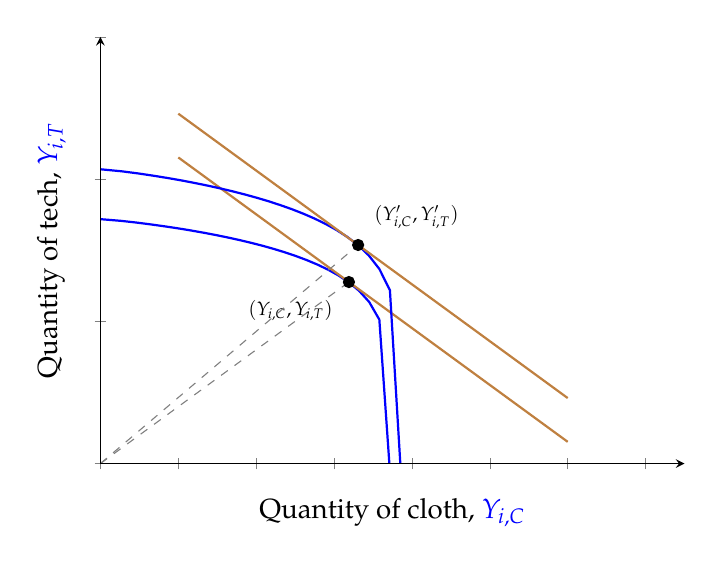
\begin{tikzpicture}
    \pgfmathsetmacro{\alpha}{0.5}
    \pgfmathsetmacro{\betat}{5/6}
    \pgfmathsetmacro{\betac}{1/6}

    \pgfmathsetmacro{\L}{1}
    \pgfmathsetmacro{\K}{1}

    \pgfmathsetmacro{\Lc}{\alpha*(1-\betac) / ((1-\alpha)* (1-\betat) + \alpha*(1-\betac)) * \L}
    \pgfmathsetmacro{\Kc}{\alpha*(\betac) / ((1-\alpha)* (\betat) + \alpha*(\betac)) * \K}
    \pgfmathsetmacro{\Lt}{\L - \Lc}
    \pgfmathsetmacro{\Kt}{\K - \Kc}

    \pgfmathsetmacro{\wr}{ \K / \L * (\alpha*(1-\betac) + (1-\alpha)*(1-\betat))/(\alpha * \betac + (1-\alpha)*\betat)  }

    \pgfmathsetmacro{\P}{ ( ((1-\betat)^(1-\betat) * \betat^(\betat)) / ((1-\betac)^(1-\betac) * \betac^(\betac)) ) * (\wr)^(\betat-\betac)  }
    
    \pgfmathsetmacro{\Yc}{ \Kc^(\betac) * \Lc^(1-\betac) }
    \pgfmathsetmacro{\Yt}{ \Kt^(\betat) * \Lt^(1-\betat) }

    \pgfmathsetmacro{\U}{(\Yc^(\alpha))*(\Yt^(1 - \alpha))}
    \pgfmathsetmacro{\expo}{(1 - \alpha)/\alpha}
    \pgfmathsetmacro{\A}{\U^(1/\alpha)}
    
    \pgfmathsetmacro{\Kk}{1.25}

    \pgfmathsetmacro{\Lck}{\alpha*(1-\betac) / ((1-\alpha)* (1-\betat) + \alpha*(1-\betac)) * \L}
    \pgfmathsetmacro{\Kck}{\alpha*(\betac) / ((1-\alpha)* (\betat) + \alpha*(\betac)) * \Kk}
    \pgfmathsetmacro{\Ltk}{\L - \Lck}
    \pgfmathsetmacro{\Ktk}{\Kk - \Kck}

    \pgfmathsetmacro{\wrk}{ \wr  }

    \pgfmathsetmacro{\Pk}{ ( ((1-\betat)^(1-\betat) * \betat^(\betat)) / ((1-\betac)^(1-\betac) * \betac^(\betac)) ) * (\wrk)^(\betat-\betac)  }
    
    \pgfmathsetmacro{\Yck}{ \Kck^(\betac) * \Lck^(1-\betac) }
    \pgfmathsetmacro{\Ytk}{ \Ktk^(\betat) * \Ltk^(1-\betat) }


    \pgfmathsetmacro{\Uk}{(\Yck^(\alpha))*(\Ytk^(1 - \alpha))}
    
    % Compute prefactor for indifference curve: Qc = A * Qr^(- (1 - alpha)/alpha)
    \pgfmathsetmacro{\Ak}{\Uk^(1/\alpha)}
    
    \centering
    \begin{axis}[
        ylabel={Quantity of tech, $\textcolor{blue}{Y_{i,T}}$},
        xlabel={Quantity of cloth, $\textcolor{blue}{Y_{i,C}}$},
        ymin=0, ymax=\L+.5,
        xmin=0, xmax=\L+.5,
        yticklabel=\empty,
        xticklabel=\empty,
        axis lines=left,
        enlargelimits=false,
        clip=false,
        axis on top,
        scaled x ticks=false,
        width=9cm, height=7cm,
        title style={font=\bfseries}
    ]
    
    % PPF: Q_C = (L/a_C) - (a_R/a_C) * Q_R
    \addplot[blue, thick, domain=0:1] ({ \Kc^(\betac) * (\L-x)^(1-\betac)}, { \Kt^(\betat) * (x)^(1-\betat)});
    \pgfmathsetmacro{\c}{ \Yt + \P * \Yc }
    \addplot[thick, brown, domain=0.2:1.2] { \c - \P*x};
    

    % Equilibrium point
    \addplot[only marks, mark=*, color=black, mark size=2pt] coordinates {(\Yc, \Yt)};
    \addplot[dashed, gray] coordinates {(0,0) (\Yc, \Yt) };
    \node at (axis cs:\Yc - .15,\Yt - 0.1) {\scriptsize $(Y_{i,C},Y_{i,T})$};
        
    \addplot[blue, thick, domain=0:1] ({ \Kck^(\betac) * (\L-x)^(1-\betac)}, { \Ktk^(\betat) * (x)^(1-\betat)});
    \pgfmathsetmacro{\ck}{ \Ytk + \Pk * \Yck }
    \addplot[thick, brown, domain=0.2:1.2] { \ck - \Pk*x};
    
    
    % Equilibrium point
    \addplot[only marks, mark=*, color=black, mark size=2pt] coordinates {(\Yck, \Ytk)};
    \addplot[dashed, gray] coordinates {(0,0) (\Yck, \Ytk) };
    \node at (axis cs:\Yck + .15,\Ytk+ 0.1) {\scriptsize $(Y'_{i,C},Y'_{i,T})$};

    
    \end{axis}

\end{tikzpicture}
    
\end{parts}

\question \textbf{Heckscher--Ohlin Theorem: Trade Patterns}

Assume two countries, Home ($H$) and Foreign ($F$), share identical technologies and preferences, but $K_H/L_H > K_F/L_F$.

\begin{parts}
    \part Which country exports which good? Explain using the H--O theorem.

    \textcolor{red}{Home is relatively capital abundant $\Rightarrow$ exports the capital-intensive good ($T$) and imports the labor-intensive good ($C$). Foreign does the opposite.}

    \part Use a diagram like Figure~4 from the handout to illustrate the production, consumption, exports, and imports of both countries.

\begin{figure}[htbp!]

% California
\begin{subfigure}{0.5\linewidth}
\resizebox{\linewidth}{!}{%
    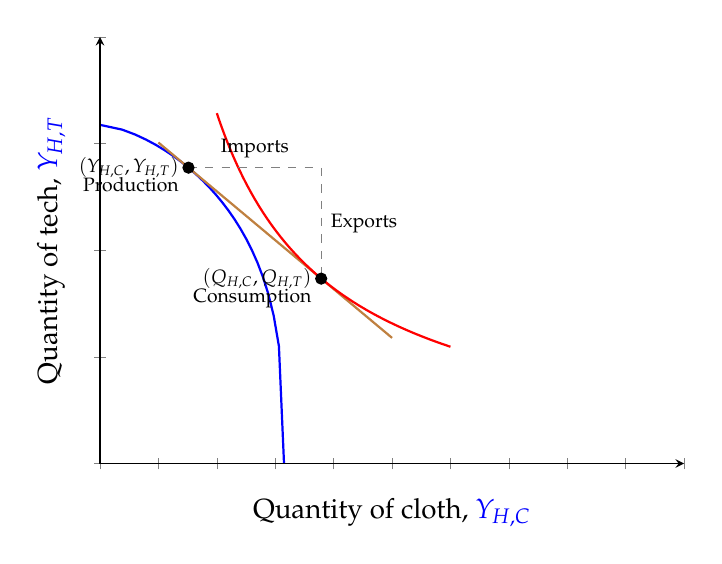
\begin{tikzpicture}
    \pgfmathsetmacro{\alpha}{0.5}
    \pgfmathsetmacro{\betat}{2/3}
    \pgfmathsetmacro{\betac}{1/3}

    \pgfmathsetmacro{\Phi}{((1-\betat)^(1-\betat))*((\betat)^\betat)/
             ((1-\betac)^(1-\betac))*((\betac)^\betac)}
    \pgfmathsetmacro{\aC}{\betac/(1-\betac)}
    \pgfmathsetmacro{\aT}{\betat/(1-\betat)}
    \pgfmathsetmacro{\d}{\aC-\aT}

    
    \pgfmathsetmacro{\L}{1}
    \pgfmathsetmacro{\K}{2.25}
    \pgfmathsetmacro{\Kk}{1.5}

   \pgfmathsetmacro{\wrk}{ \K / \L * (\alpha*(1-\betac) + (1-\alpha)*(1-\betat))/(\alpha * \betac + (1-\alpha)*\betat)  }
    \pgfmathsetmacro{\wr}{  \Kk / \L * (\alpha*(1-\betac) + (1-\alpha)*(1-\betat))/(\alpha * \betac + (1-\alpha)*\betat) }

    \pgfmathsetmacro{\P}{ ( ((1-\betat)^(1-\betat) * \betat^(\betat)) / ((1-\betac)^(1-\betac) * \betac^(\betac)) ) * (\wr)^(\betat-\betac)  }

       
    \pgfmathsetmacro{\Lc}{ (\K - \aT*\wr*\L)/(\d * \wr) }
    \pgfmathsetmacro{\Kc}{\aC * \wr * \Lc}
    \pgfmathsetmacro{\Lt}{\L - \Lc}
    \pgfmathsetmacro{\Kt}{\K - \Kc}
   
    \pgfmathsetmacro{\Yc}{ \Kc^(\betac) * \Lc^(1-\betac) }
    \pgfmathsetmacro{\Yt}{ \Kt^(\betat) * \Lt^(1-\betat) }

    

    \pgfmathsetmacro{\I}{ \P * \Yc + \Yt }
    \pgfmathsetmacro{\Qc}{(1-\alpha)/\P * \I}
    \pgfmathsetmacro{\Qt}{(\alpha) * \I}

    \pgfmathsetmacro{\U}{(\Qt^(\alpha))*(\Qc^(1 - \alpha))}
    \pgfmathsetmacro{\expo}{(1 - \alpha)/\alpha}
    \pgfmathsetmacro{\A}{\U^(1/\alpha)}

    
    
    \centering
    \begin{axis}[
        ylabel={Quantity of tech, $\textcolor{blue}{Y_{H,T}}$},
        xlabel={Quantity of cloth, $\textcolor{blue}{Y_{H,C}}$},
        ymin=0, ymax=2,
        xmin=0, xmax=2,
        yticklabel=\empty,
        xticklabel=\empty,
        axis lines=left,
        enlargelimits=false,
        clip=false,
        axis on top,
        scaled x ticks=false,
        width=9cm, height=7cm,
        title style={font=\bfseries}
    ]
    
    % PPF: Q_C = (L/a_C) - (a_R/a_C) * Q_R
    \addplot[blue, thick, domain=0:1] ({ \Kc^(\betac) * (\L-x)^(1-\betac)}, { \Kt^(\betat) * (x)^(1-\betat)});
    \pgfmathsetmacro{\c}{ \Yt + \P * \Yc }
    \addplot[thick, brown, domain=0.2:1] { \c - \P*x};
    
    \addplot[thick, red, domain=0.4:1.2, samples=100] {\A * x^(-\expo)};

    % Equilibrium point
    \addplot[only marks, mark=*, color=black, mark size=2pt] coordinates {(\Yc, \Yt)};
    \node[anchor = north east] at (axis cs:\Yc,\Yt) {\scriptsize Production};
    \node[anchor = east] at (axis cs:\Yc,\Yt) {\scriptsize $(Y_{H,C},Y_{H,T})$};
        
    \addplot[only marks, mark=*, color=black, mark size=2pt] coordinates {(\Qc, \Qt)};
    \node[anchor = north east] at (axis cs:\Qc,\Qt) {\scriptsize Consumption};
    \node[anchor = east] at (axis cs:\Qc,\Qt) {\scriptsize $(Q_{H,C},Q_{H,T})$};

    \addplot[dashed, gray] coordinates {(\Yc, \Yt) (\Qc, \Yt)  (\Qc, \Qt)};
    \node[anchor = south] at (axis cs:{\Yc + (\Qc-\Yc)/2}, \Yt) {\scriptsize Imports};
    \node[anchor = west] at (axis cs:\Qc, {\Yt + (\Qt-\Yt)/2}) {\scriptsize Exports};
    
    \end{axis}

\end{tikzpicture}
}
\end{subfigure}
%
% Colombia
\begin{subfigure}{0.5\textwidth}
\resizebox{\linewidth}{!}{%

    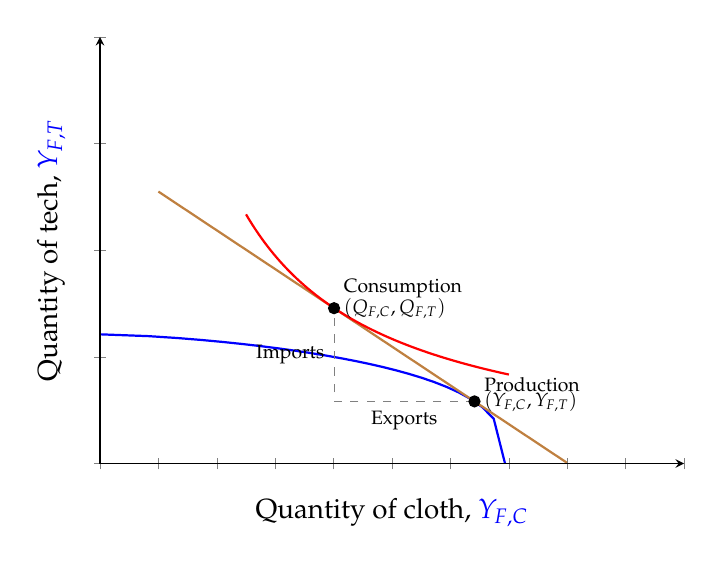
\begin{tikzpicture}
    \pgfmathsetmacro{\alpha}{0.5}
    \pgfmathsetmacro{\betat}{2/3}
    \pgfmathsetmacro{\betac}{1/3}

    \pgfmathsetmacro{\Phi}{((1-\betat)^(1-\betat))*((\betat)^\betat)/
             ((1-\betac)^(1-\betac))*((\betac)^\betac)}
    \pgfmathsetmacro{\aC}{\betac/(1-\betac)}
    \pgfmathsetmacro{\aT}{\betat/(1-\betat)}
    \pgfmathsetmacro{\d}{\aC-\aT}

    
    \pgfmathsetmacro{\L}{2}
    \pgfmathsetmacro{\K}{1}
    \pgfmathsetmacro{\Kk}{1.5}

   \pgfmathsetmacro{\wrk}{ \K / \L * (\alpha*(1-\betac) + (1-\alpha)*(1-\betat))/(\alpha * \betac + (1-\alpha)*\betat)  }
    \pgfmathsetmacro{\wr}{  \Kk / \L * (\alpha*(1-\betac) + (1-\alpha)*(1-\betat))/(\alpha * \betac + (1-\alpha)*\betat) }

    \pgfmathsetmacro{\P}{ ( ((1-\betat)^(1-\betat) * \betat^(\betat)) / ((1-\betac)^(1-\betac) * \betac^(\betac)) ) * (\wr)^(\betat-\betac)  }

       
    \pgfmathsetmacro{\Lc}{ (\K - \aT*\wr*\L)/(\d * \wr) }
    \pgfmathsetmacro{\Kc}{\aC * \wr * \Lc}
    \pgfmathsetmacro{\Lt}{\L - \Lc}
    \pgfmathsetmacro{\Kt}{\K - \Kc}
   
    \pgfmathsetmacro{\Yc}{ \Kc^(\betac) * \Lc^(1-\betac) }
    \pgfmathsetmacro{\Yt}{ \Kt^(\betat) * \Lt^(1-\betat) }

    

    \pgfmathsetmacro{\I}{ \P * \Yc + \Yt }
    \pgfmathsetmacro{\Qc}{(1-\alpha)/\P * \I}
    \pgfmathsetmacro{\Qt}{(\alpha) * \I}

    \pgfmathsetmacro{\U}{(\Qt^(\alpha))*(\Qc^(1 - \alpha))}
    \pgfmathsetmacro{\expo}{(1 - \alpha)/\alpha}
    \pgfmathsetmacro{\A}{\U^(1/\alpha)}

    
    
    \centering
    \begin{axis}[
        ylabel={Quantity of tech, $\textcolor{blue}{Y_{F,T}}$},
        xlabel={Quantity of cloth, $\textcolor{blue}{Y_{F,C}}$},
        ymin=0, ymax=2,
        xmin=0, xmax=2,
        yticklabel=\empty,
        xticklabel=\empty,
        axis lines=left,
        enlargelimits=false,
        clip=false,
        axis on top,
        scaled x ticks=false,
        width=9cm, height=7cm,
        title style={font=\bfseries}
    ]
    
    % PPF: Q_C = (L/a_C) - (a_R/a_C) * Q_R
    \addplot[blue, thick, domain=0:2] ({ \Kc^(\betac) * (\L-x)^(1-\betac)}, { \Kt^(\betat) * (x)^(1-\betat)});
    \pgfmathsetmacro{\c}{ \Yt + \P * \Yc }
    \addplot[thick, brown, domain=0.2:1.6] { \c - \P*x};
    
    \addplot[thick, red, domain=0.5:1.4, samples=100] {\A * x^(-\expo)};

    % Equilibrium point
    \addplot[only marks, mark=*, color=black, mark size=2pt] coordinates {(\Yc, \Yt)};
    \node[anchor = south west] at (axis cs:\Yc,\Yt) {\scriptsize Production};
    \node[anchor = west] at (axis cs:\Yc,\Yt) {\scriptsize $(Y_{F,C},Y_{F,T})$};
        
    \addplot[only marks, mark=*, color=black, mark size=2pt] coordinates {(\Qc, \Qt)};
    \node[anchor = south west] at (axis cs:\Qc,\Qt) {\scriptsize Consumption};
    \node[anchor = west] at (axis cs:\Qc,\Qt) {\scriptsize $(Q_{F,C},Q_{F,T})$};

    \addplot[dashed, gray] coordinates {(\Yc, \Yt) (\Qc, \Yt)  (\Qc, \Qt)};
    \node[anchor = north] at (axis cs:{\Yc + (\Qc-\Yc)/2}, \Yt) {\scriptsize Exports};
    \node[anchor = east] at (axis cs:\Qc, {\Yt + (\Qt-\Yt)/2}) {\scriptsize Imports};
    
    \end{axis}

\end{tikzpicture}
}

\end{subfigure}

\caption{The Result of Hecksher-Ohlin Trade}\label{fig: consumption-trade}

\end{figure}

\end{parts}

\newpage

\question \textbf{Factor Price Equalization}

\begin{parts}
    \part Using the expression derived in class,
    \[
    \frac{P_C}{P_T} = \text{constant} \times \left(\frac{w}{r}\right)^{\beta_T-\beta_C},
    \]
    explain why, under free trade, relative factor prices equalize across countries.

    \textcolor{red}{Under free trade, countries face the same $\tfrac{P_C}{P_T}$; with common technologies and both goods produced, the mapping from $\tfrac{P_C}{P_T}$ to $\tfrac{w}{r}$ is \emph{one-to-one}. Hence $\tfrac{w}{r}$ must be equalized across countries (FPE).}

    \part Discuss at least two reasons why complete factor price equalization may fail in the real world.

    \textcolor{red}{(i) Trade costs and tariffs segment goods prices; (ii) technology differences; (iii) non-diversification (corner solutions); (iv) factor intensity reversals; (v) measurement and quality differences in goods/factors.}
\end{parts}


\end{questions}

\end{document}
